\documentclass{beamer}

%\usetheme{AnnArbor}
\usetheme{Boadilla}
\usecolortheme{whale}

\usepackage[utf8]{inputenc}
\graphicspath{{../Graphics/}}

\usepackage[absolute,overlay]{textpos}
\setlength{\TPHorizModule}{1pt}
\setlength{\TPVertModule}{1pt}
\usepackage{calc}

\usepackage{lipsum}

%Information to be included in the title page:
\title{Heat Energy Sources in Canada}
\author[Team 9 (Mcmillan-Mcgee)]
{Team 9 (Mcmillan-Mcgee): Benjamin MacAdam, Noah Bolohan, Anton Iatcenko, Ryan Thiessen, Alireza Yazdani, Yakine Bahri}
\institute[]{Math\textsuperscript{Industry}}

\date{August 2020}

\titlegraphic{
\includegraphics[width=2cm]{pims_logo.png}}



\begin{document}

\frame{\titlepage}


\begin{frame}
\frametitle{Team Members}

\begin{minipage}[c]{0.15\textwidth}
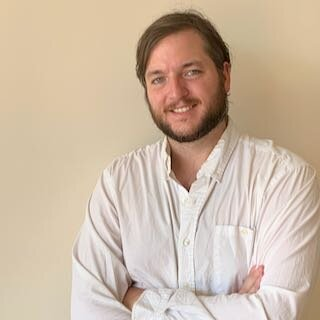
\includegraphics[width=\textwidth, trim={25pt 0pt 0pt 0pt}, clip]{TeamPics/Ben.jpg}
\end{minipage}\hspace{0.05\textwidth}%
\begin{minipage}[c]{0.8\textwidth}
{\small \textbf{Benjamin} is a PhD candidate in the programming languages lab at the University of Calgary. His research interests mainly revolve around tangent categories and their applications to differentiable programming and Lie theory. }
\end{minipage}

\vspace{10pt}
\begin{minipage}[c]{0.15\textwidth}

\includegraphics[width=\textwidth, trim={180pt 0pt 180pt 0pt}, clip]{TeamPics/Noah.jpg}
\end{minipage}\hspace{0.05\textwidth}%
\begin{minipage}[c]{0.8\textwidth}
{\small \textbf{Noah} is a recent graduate student from the University of Ottawa studying the effects of seasonality on predator-prey scenarios. His work focuses on bistability and bifurcations in ordinary differential equation models using MATLAB and XPPAUTO. His interests lie in mathematical ecology and mathematical modelling.}
\end{minipage}

\vspace{10pt}
\begin{minipage}[c]{0.15\textwidth}
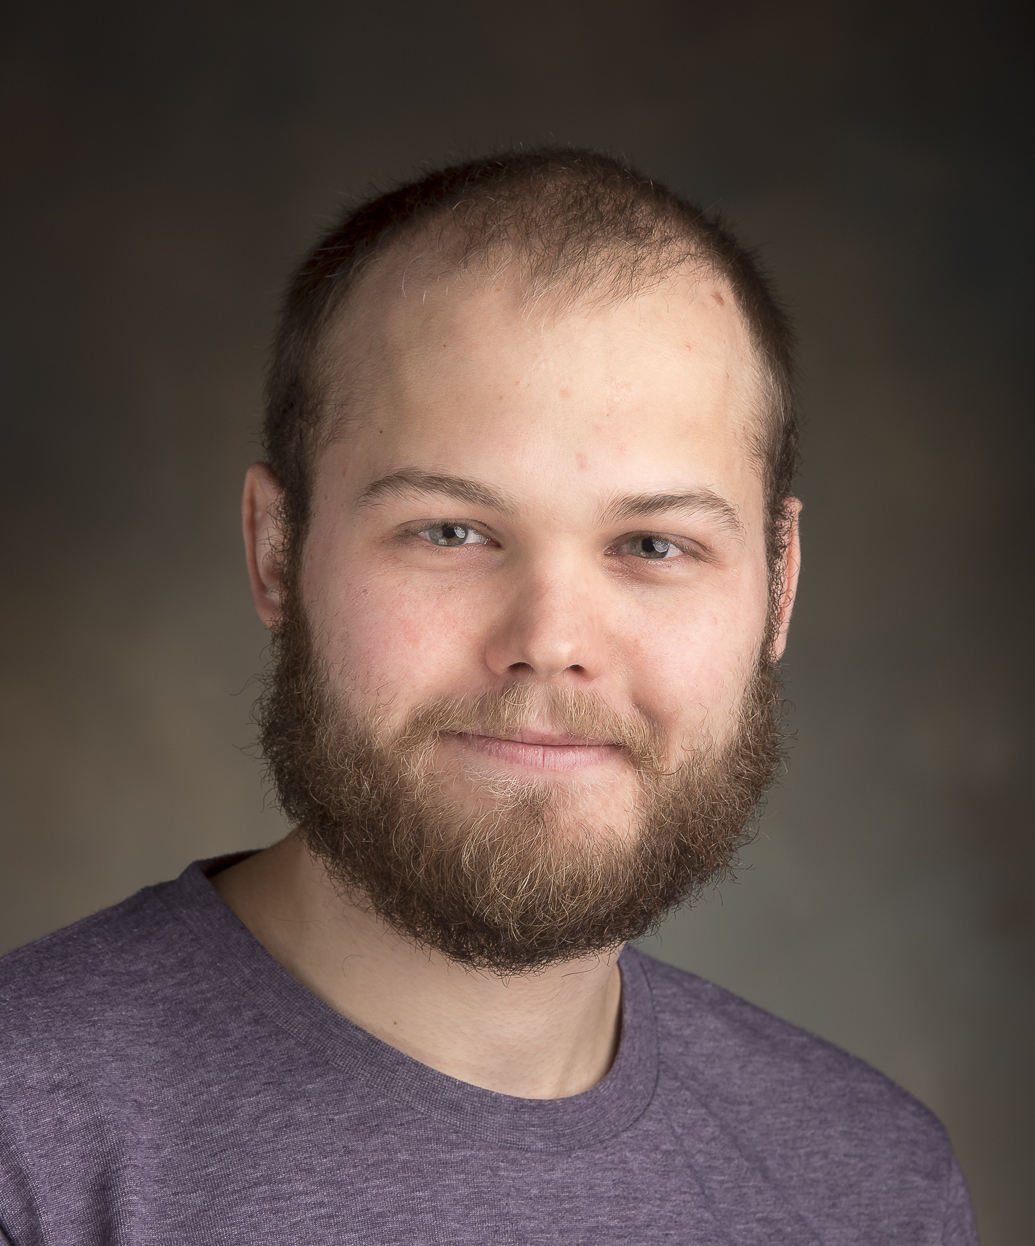
\includegraphics[width=\textwidth, trim={70pt 170pt 70pt 100pt}, clip]{TeamPics/anton.jpg}
\end{minipage}\hspace{0.05\textwidth}%
\begin{minipage}[c]{0.8\textwidth}
{\small \textbf{Anton} is a PhD student at the Departmen of Mathematics at SFU. His background is in the areas of pde analysis and kinetic theory, while the current interests are leaning towards numerical solutions of partial differential equations and mathematical modelling. }
\end{minipage}

\end{frame}


\begin{frame}
\frametitle{Team Members}


\begin{minipage}[c]{0.15\textwidth}
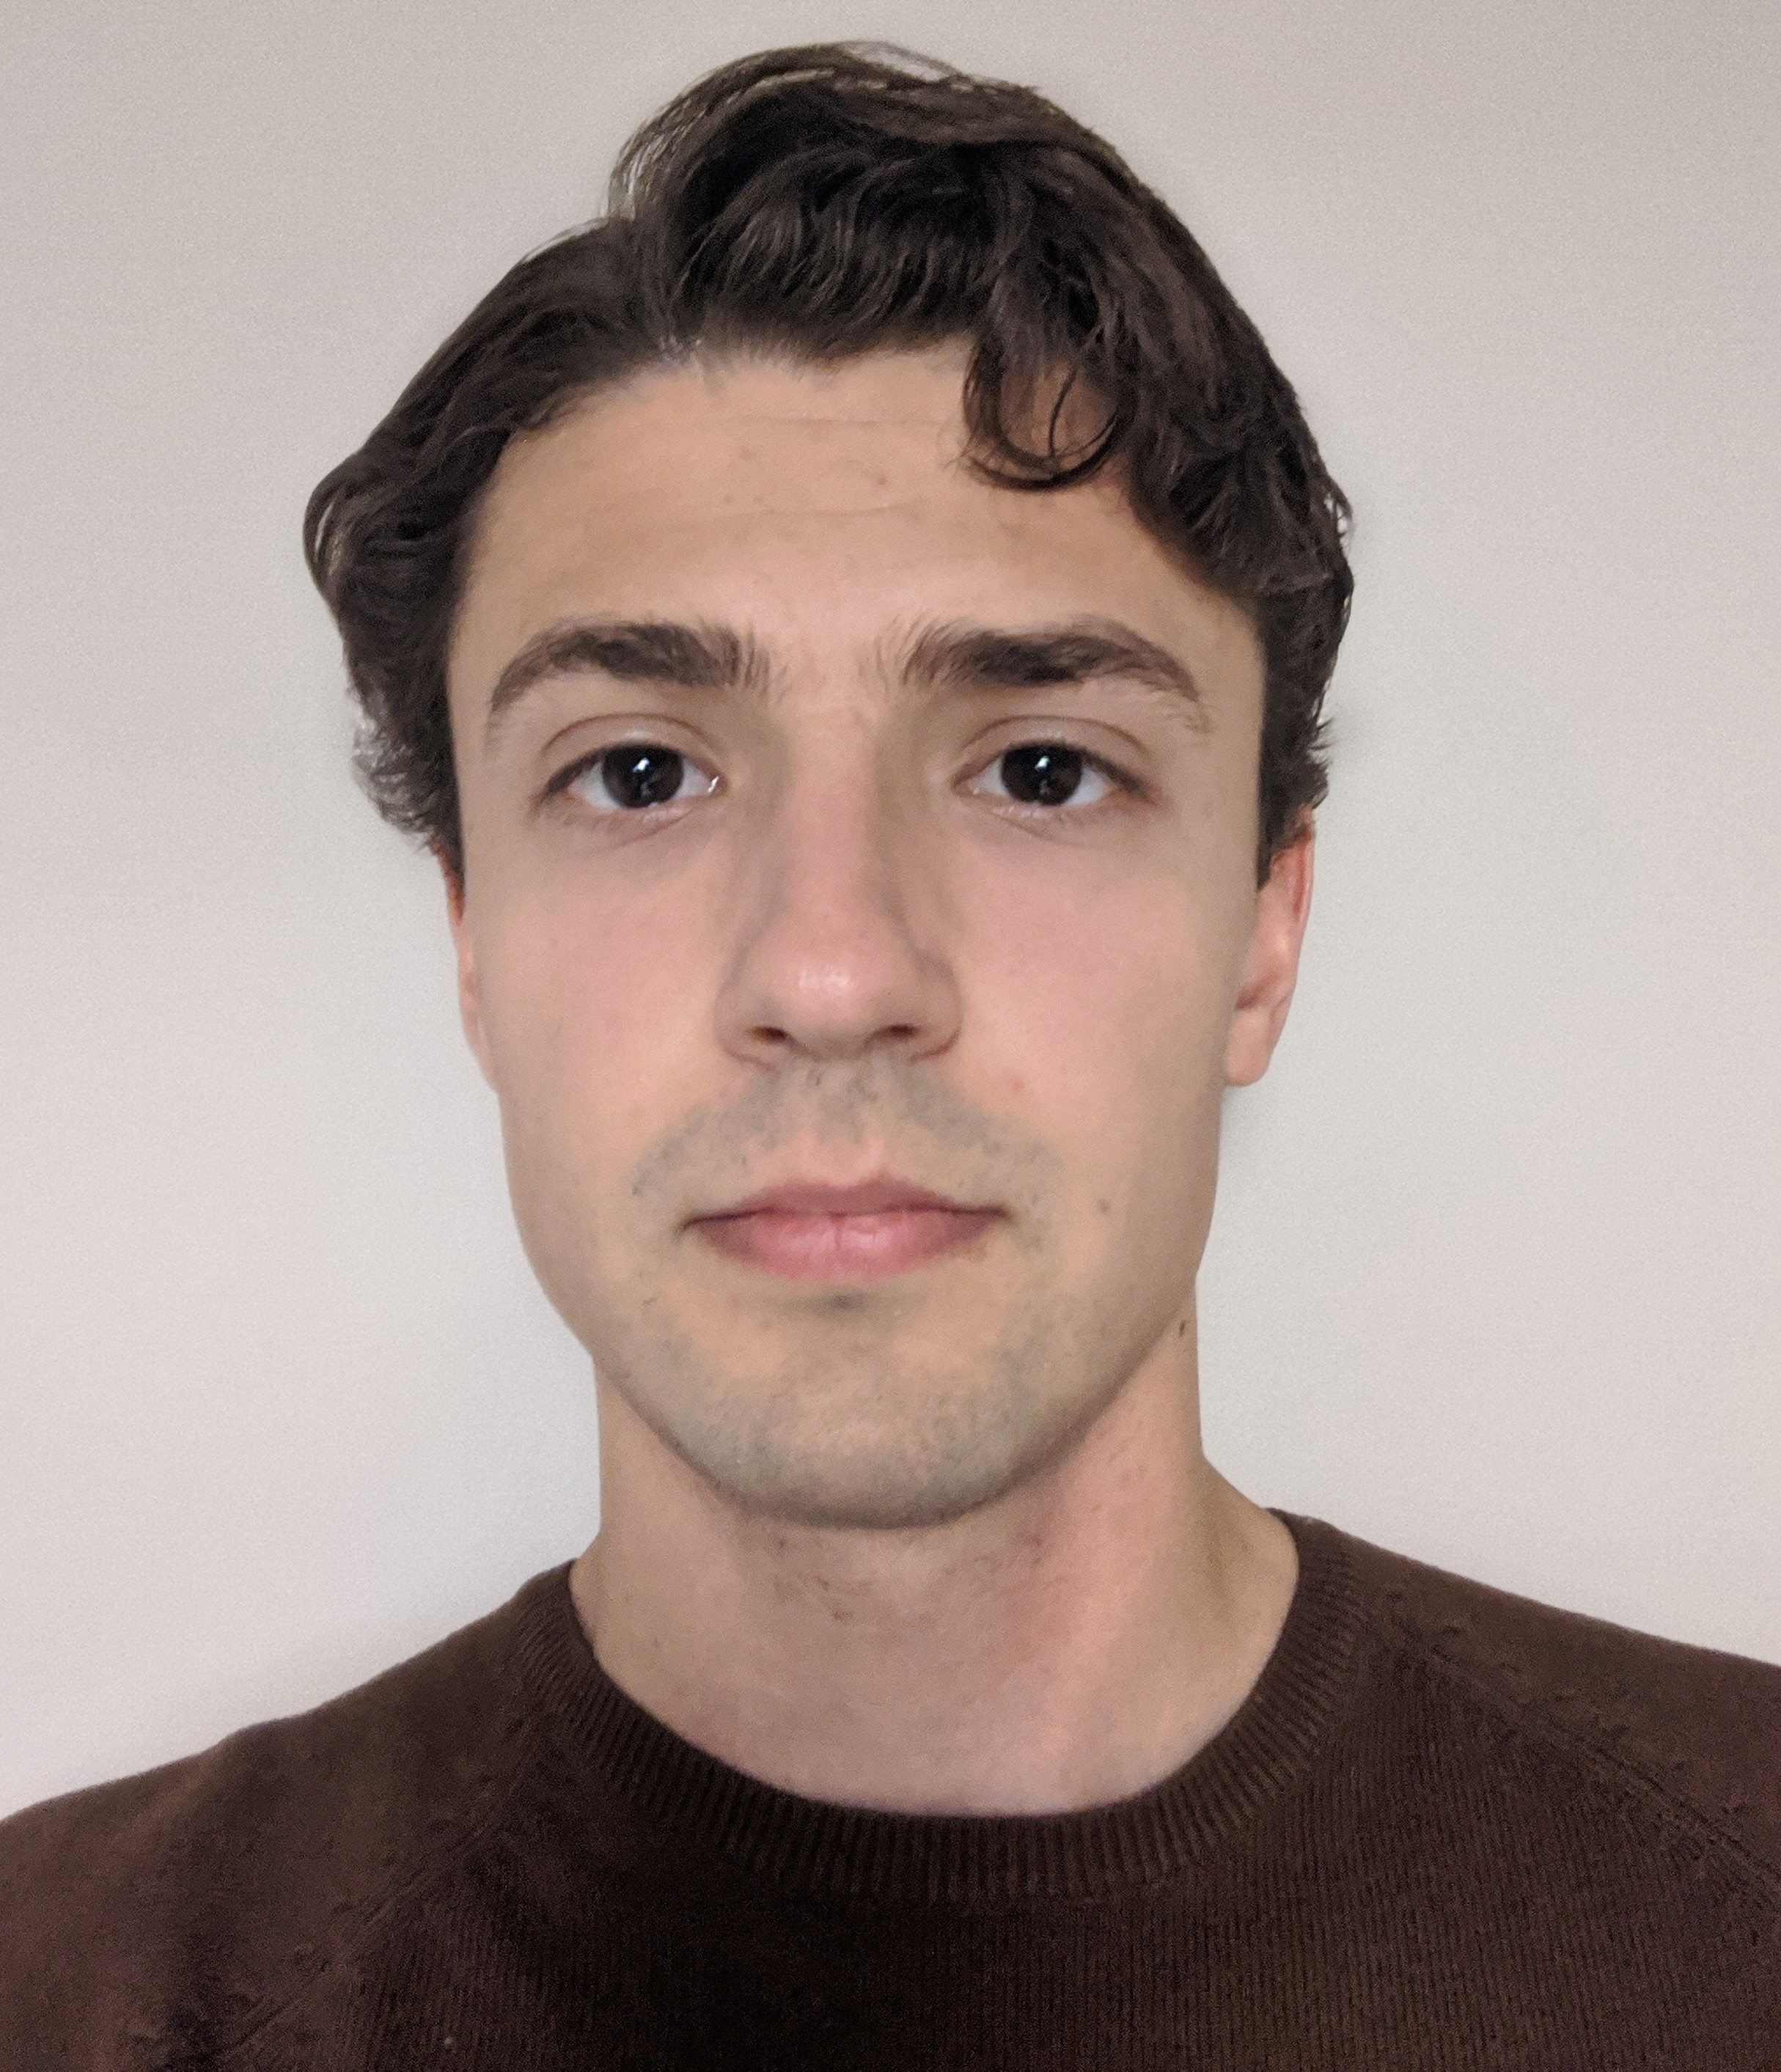
\includegraphics[width=\textwidth, trim={70pt 170pt 70pt 100pt}, clip]{TeamPics/ryan.jpg}
\end{minipage}\hspace{0.05\textwidth}%
\begin{minipage}[c]{0.8\textwidth}
{\small \textbf{Ryan} is a Master’s student at the University of Alberta, working on an analysis of scaling limits of the kinetic chemotaxis equation. He has a background in Physics, Mathematical Biology, and Numerical Methods.}
\end{minipage}


\vspace{10pt}
\begin{minipage}[c]{0.15\textwidth}
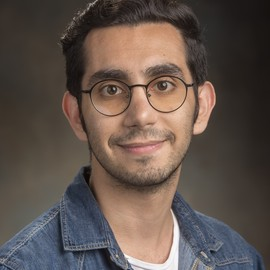
\includegraphics[width=\textwidth, trim={30pt 0pt 30pt 0pt}, clip]{TeamPics/alireza.jpg}
\end{minipage}\hspace{0.05\textwidth}%
\begin{minipage}[c]{0.8\textwidth}
{\small \textbf{Alireza} is a M.Sc. student at Mathematics department of Simon Fraser University. His background is in the areas of mechanical engineering and computational fluid dynamics, while his current research is to implement new algorithms for solving partial differential equation on surfaces using parallel computing techniques. }
\end{minipage}


\vspace{10pt}
\begin{minipage}[c]{0.15\textwidth}
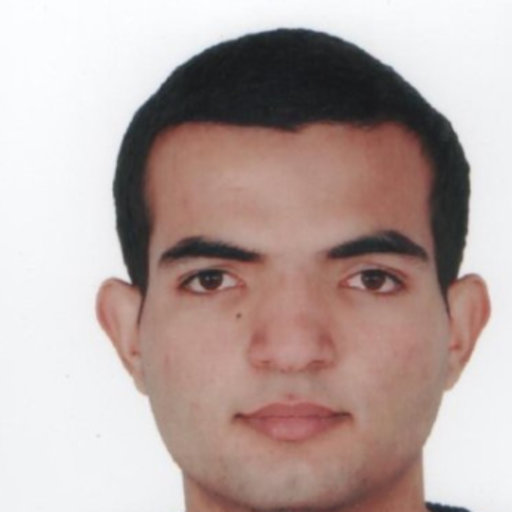
\includegraphics[width=\textwidth, trim={60pt 0pt 0pt 0pt}, clip]{TeamPics/yakine.jpg}
\end{minipage}\hspace{0.05\textwidth}%
\begin{minipage}[c]{0.8\textwidth}
{\small \textbf{Yakine} is a Postdoctoral Fellow at the University of Victoria. His broad research interests are in applied mathematics,
specifically the nonlinear PDEs arising from physics (nonlinear optics, plasma physics or micro-magnetism). The focal point of his research is the qualitative description of the dynamics including singularity formation or long-time asymptotic. 
}
\end{minipage}


\end{frame}





\begin{frame}
\frametitle{The Data Set}
\textbf{Primary heating systems and types of energy sources}\\
The table contains 2304 series, with data for the years 2013, 2015 and 2017. 
It contains data described by the following dimensions:
\begin{itemize}
\item Geography (48 items: Canada; Newfoundland and Labrador; Prince Edward Island; Nova Scotia; ...)
\item Primary heating system and type of energy (48 items: All primary heating systems; Electricity; Natural gas; Oil; ...).
\end{itemize}
\textbf{Source:} {\scriptsize https://open.canada.ca/data/en/dataset/ec3282b6-013f-41b1-aa63-24ad8bda79ee}
\end{frame}


\begin{frame}
\frametitle{Primary heating types in Canada: 2013-2017}
\begin{center}
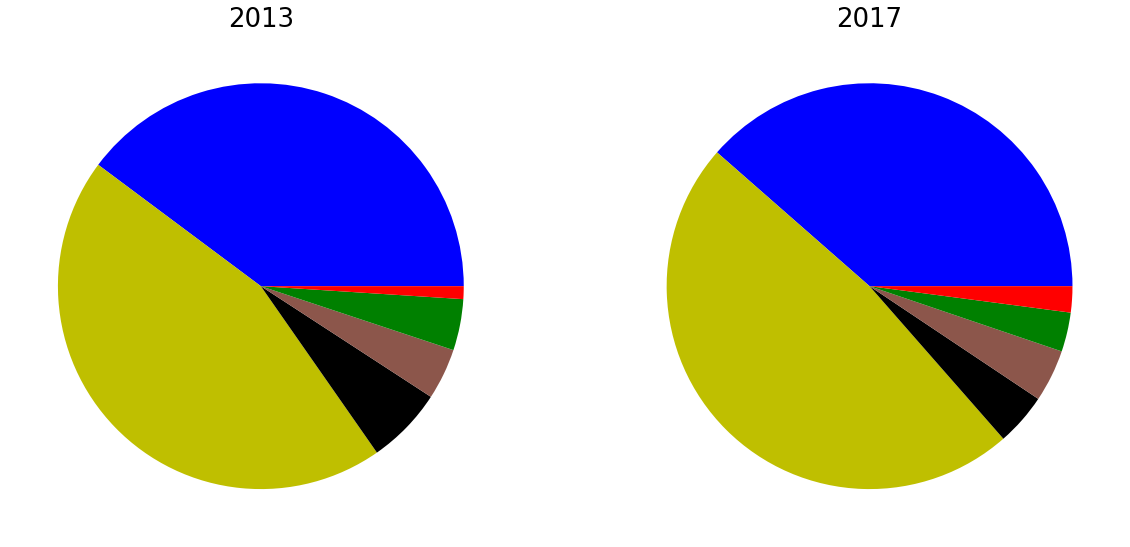
\includegraphics[width=\textwidth]{Canada20132017.png}\\
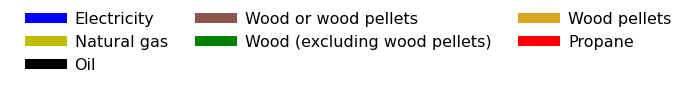
\includegraphics[width=0.8\linewidth]{leg_bar.png}
\end{center}
\end{frame}



\begin{frame}
\frametitle{Data by Province}
\begin{center}
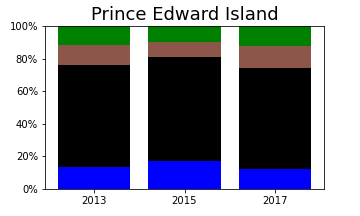
\includegraphics[width=0.5\linewidth]{pe.png}%
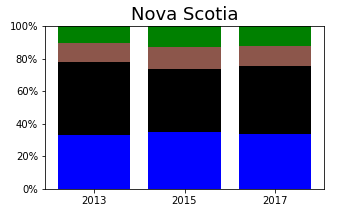
\includegraphics[width=0.5\linewidth]{ns.png}\\
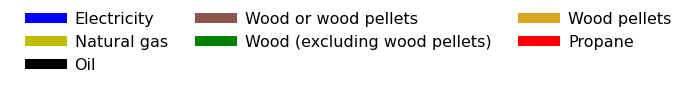
\includegraphics[width=0.8\linewidth]{leg_bar.png}
\end{center}
\end{frame}


\begin{frame}
\frametitle{Data by Province}
\vspace{-10pt}
\begin{center}
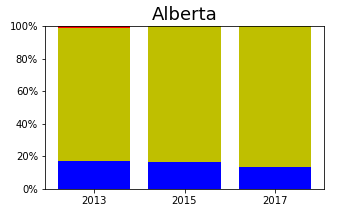
\includegraphics[width=0.48\linewidth]{ab.png}%
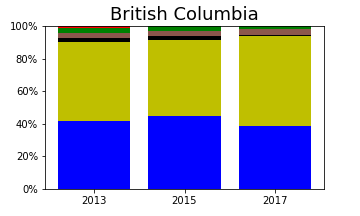
\includegraphics[width=0.48\linewidth]{bc.png}\\
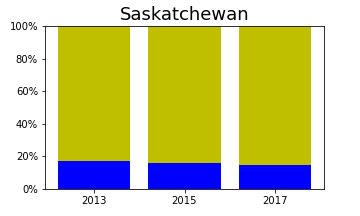
\includegraphics[width=0.48\linewidth]{sk.png}%
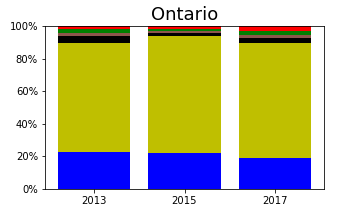
\includegraphics[width=0.48\linewidth]{on.png}\\
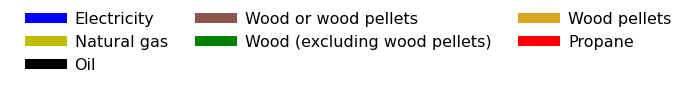
\includegraphics[width=0.9\linewidth]{leg_bar.png}
\end{center}
\end{frame}


\begin{frame}
\frametitle{Data by Province}
\vspace{-10pt}
\begin{center}
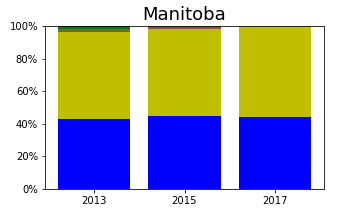
\includegraphics[width=0.48\linewidth]{mn.png}%
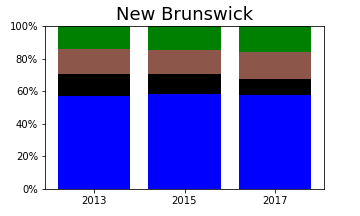
\includegraphics[width=0.48\linewidth]{nb.png}\\
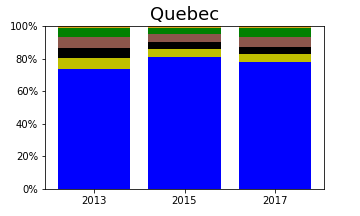
\includegraphics[width=0.48\linewidth]{qc.png}%
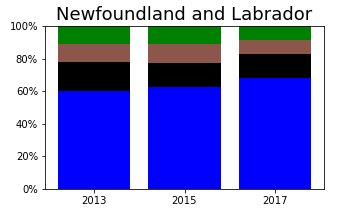
\includegraphics[width=0.48\linewidth]{nl.png}\\
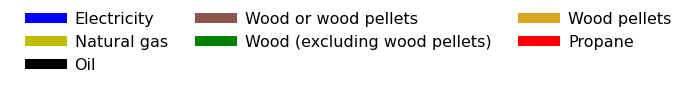
\includegraphics[width=0.9\linewidth]{leg_bar.png}
\end{center}
\end{frame}



\begin{frame}
\frametitle{Province Groupings}


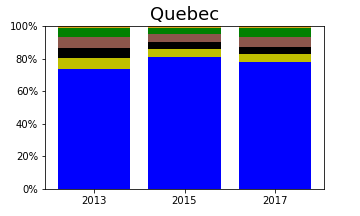
\includegraphics[width=0.33\linewidth]{qc.png}%
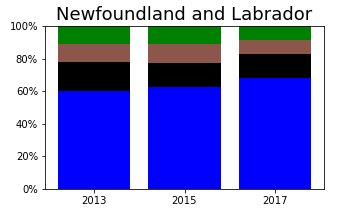
\includegraphics[width=0.33\linewidth]{nl.png}%
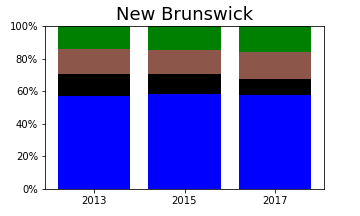
\includegraphics[width=0.33\linewidth]{nb.png}\\[10pt]
%
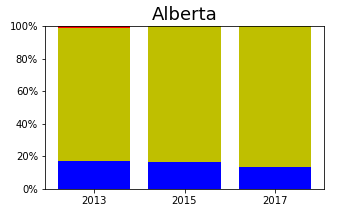
\includegraphics[width=0.33\linewidth]{ab.png}%
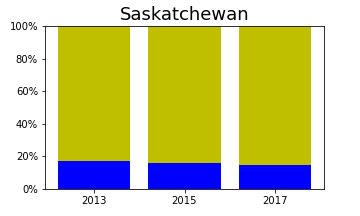
\includegraphics[width=0.33\linewidth]{sk.png}%
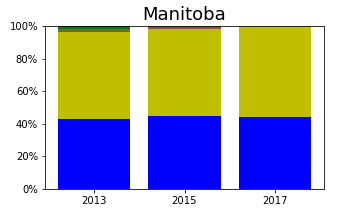
\includegraphics[width=0.33\linewidth]{mn.png}\\[10pt]
%
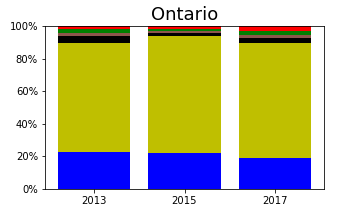
\includegraphics[width=0.25\linewidth]{on.png}%
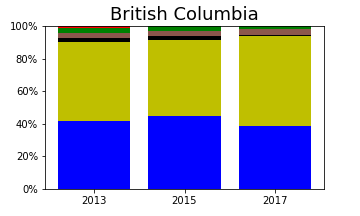
\includegraphics[width=0.25\linewidth]{bc.png}%
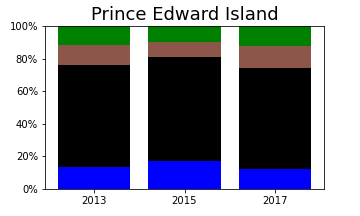
\includegraphics[width=0.25\linewidth]{pe.png}%
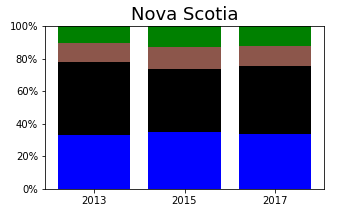
\includegraphics[width=0.25\linewidth]{ns.png}


\end{frame}





\begin{frame}
\frametitle{Cause of the Groupings: Natural Gas}
\vspace{-40pt}
\begin{center}
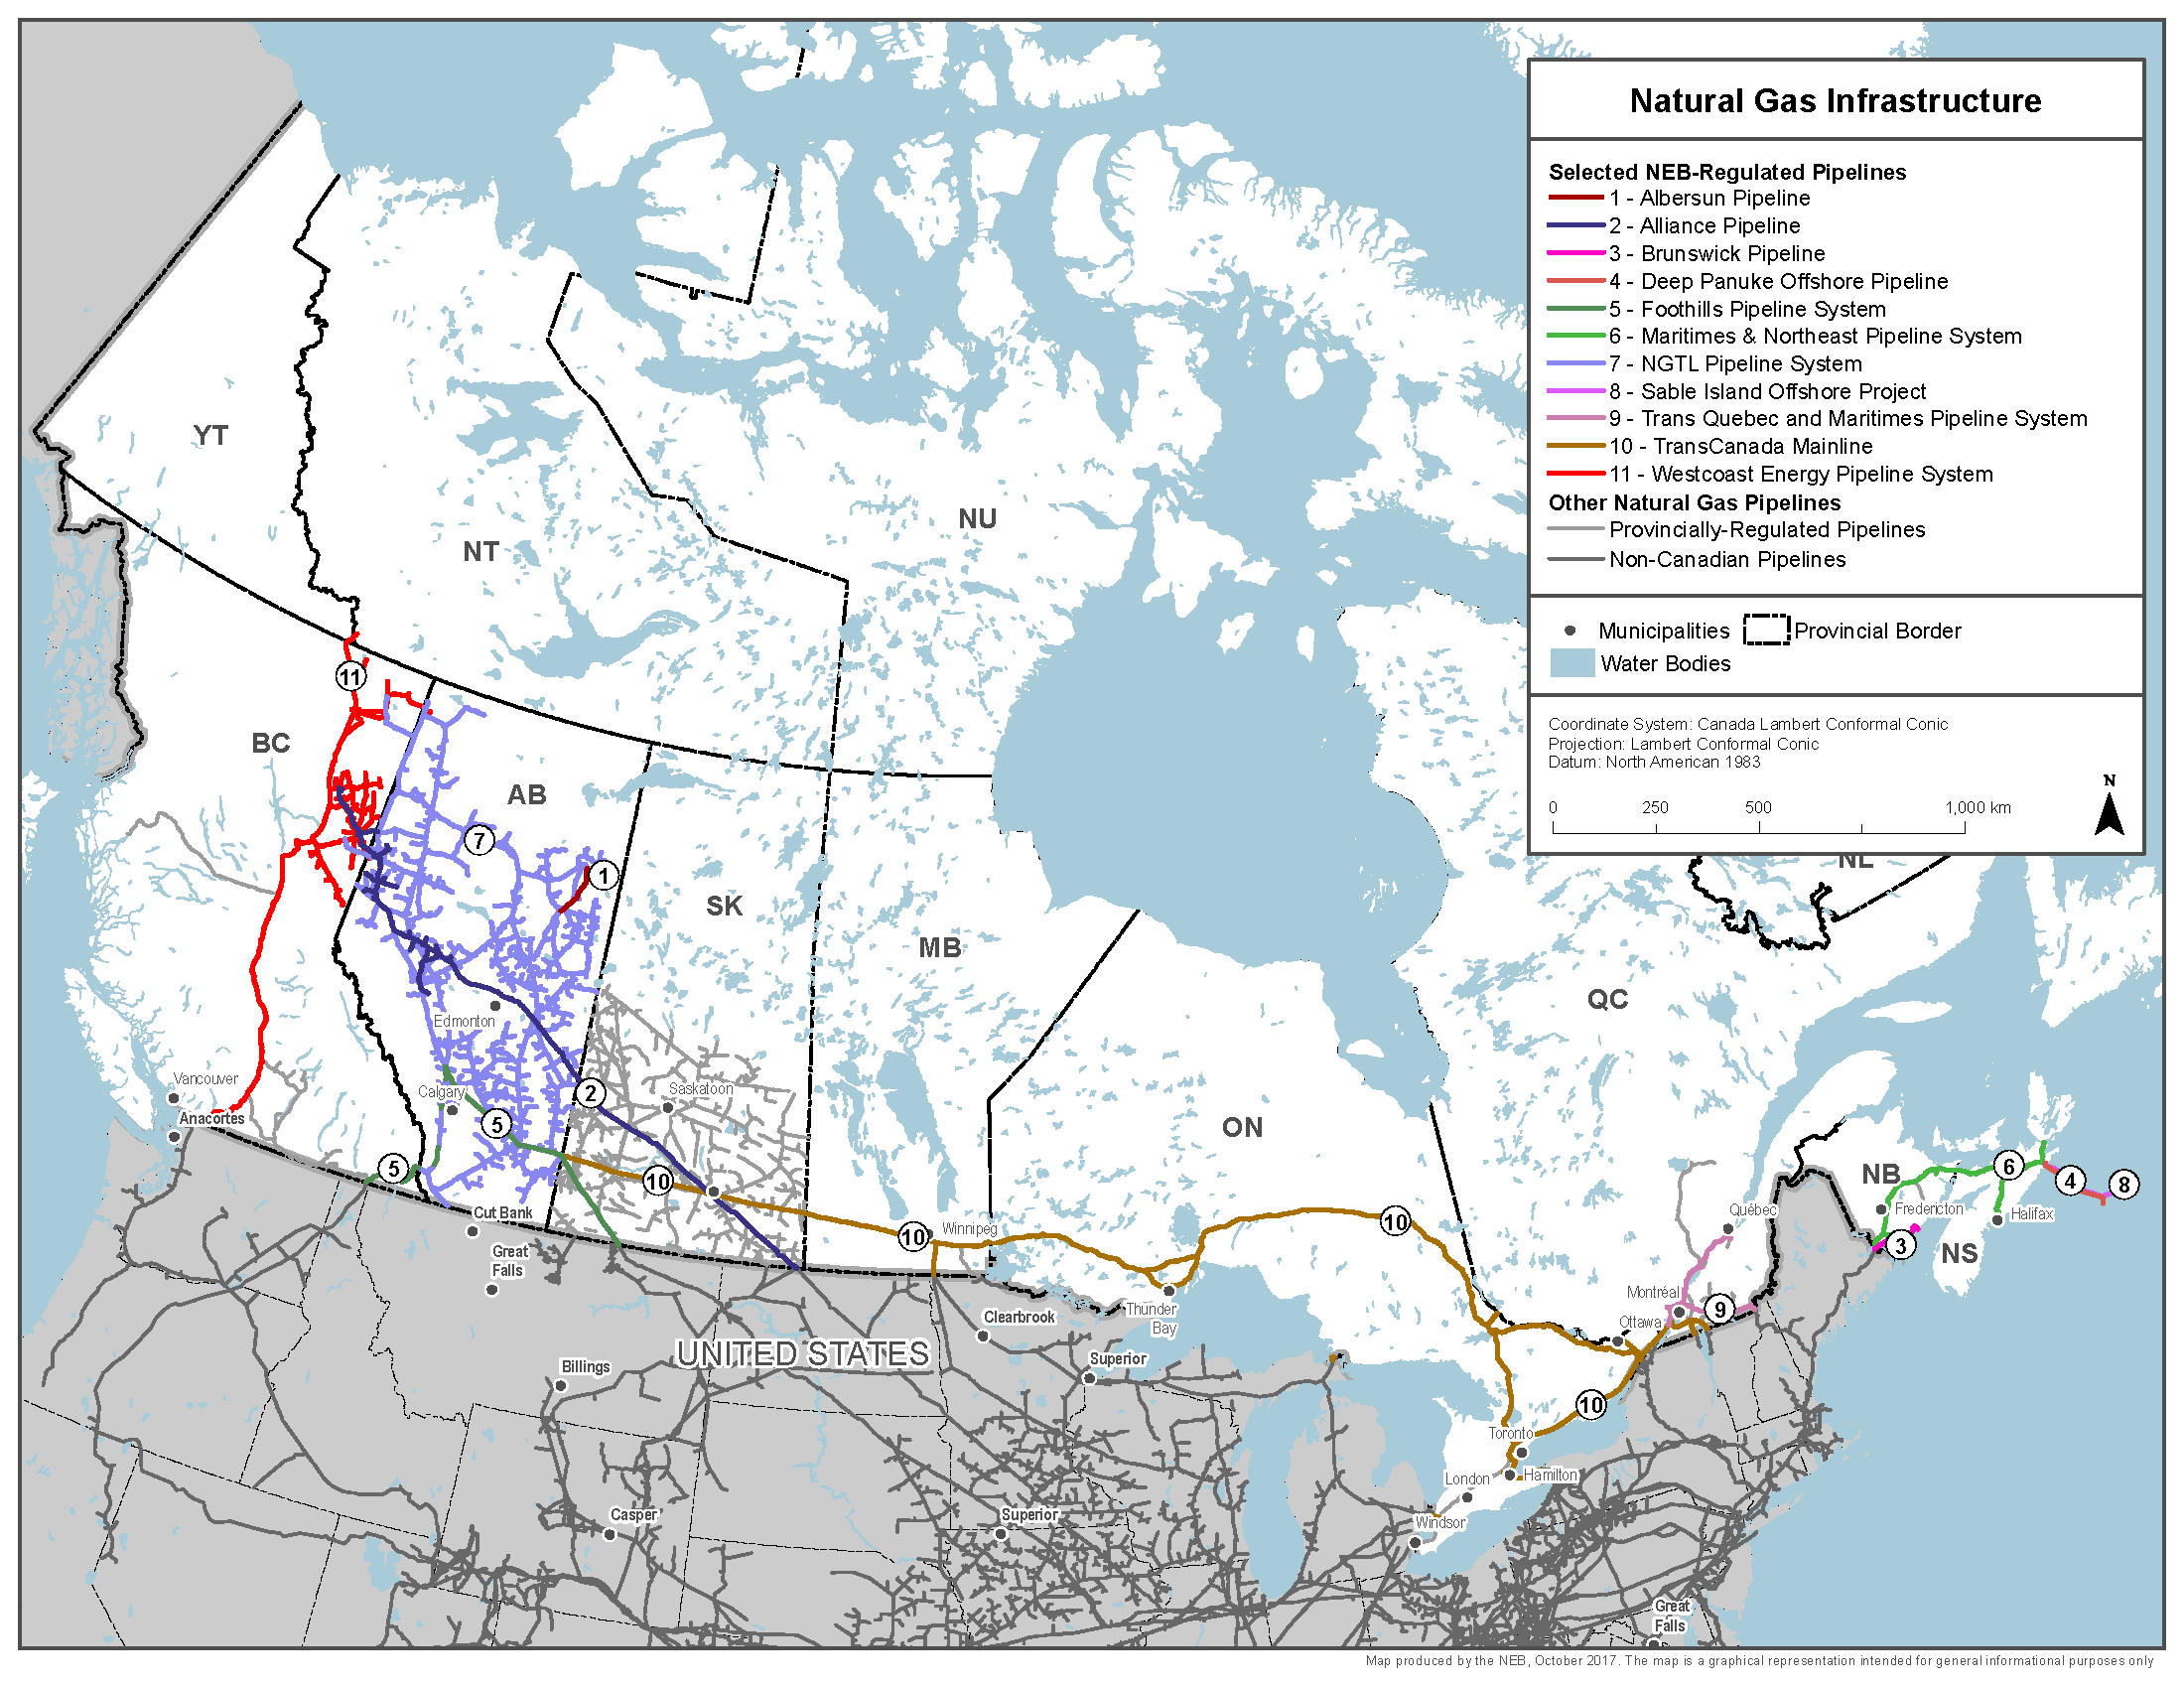
\includegraphics[width=0.9\textwidth, trim={15pt 130pt 240pt 220pt}, clip]{natural_gas_pipeline_natural_resources_canada}
\end{center} 

\begin{textblock*}{\textwidth}[0.5, 0.5](0.5\linewidth, 225pt)
\begin{itemize}
	\item SK, AB, and parts of BC have an extensive natural gas infrastructure.
	\item MB and ON have access to the natural gas TransCanada pipeline.
\end{itemize}
\end{textblock*}
\end{frame}



\begin{frame}
\frametitle{Cause of the Groupings: Natural Gas}


\begin{minipage}[b]{0.2\textwidth}
\begin{center}
\tiny{British Columbia}
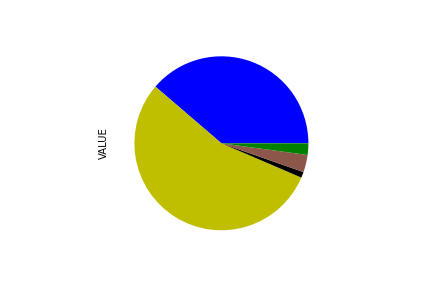
\includegraphics[width=\textwidth, trim={120pt 50pt 110pt 50pt}, clip]{../British_Columbia.png}%
\end{center}
\end{minipage}%
%
\begin{minipage}[b]{0.2\textwidth}
\begin{center}
\tiny{Alberta}
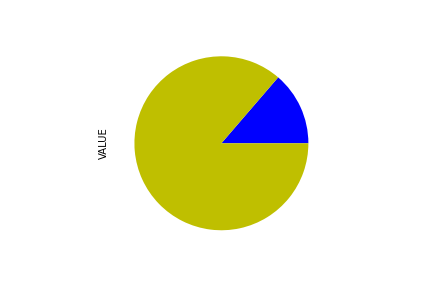
\includegraphics[width=\textwidth, trim={120pt 50pt 110pt 50pt}, clip]{../Alberta.png}%
\end{center}
\end{minipage}%
%
\begin{minipage}[b]{0.2\textwidth}
\begin{center}
\tiny{Saskatchewan}
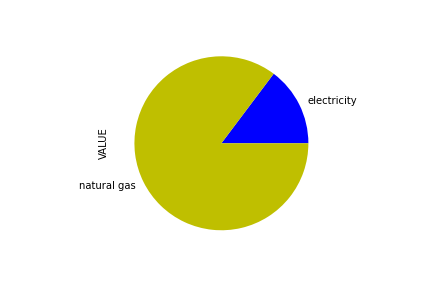
\includegraphics[width=\textwidth, trim={120pt 50pt 110pt 50pt}, clip]{../Saskatchewan.png}%
\end{center}
\end{minipage}%
%
\begin{minipage}[b]{0.2\textwidth}
\begin{center}
\tiny{Manitoba}
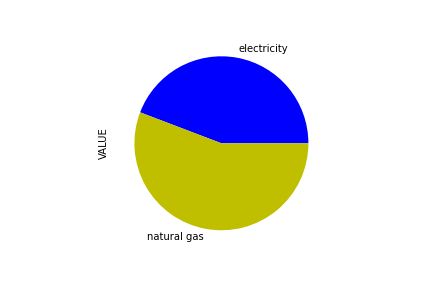
\includegraphics[width=\textwidth, trim={120pt 50pt 110pt 50pt}, clip]{../Manitoba.png}%
\end{center}
\end{minipage}%
%
\begin{minipage}[b]{0.2\textwidth}
\begin{center}
\tiny{Ontario}
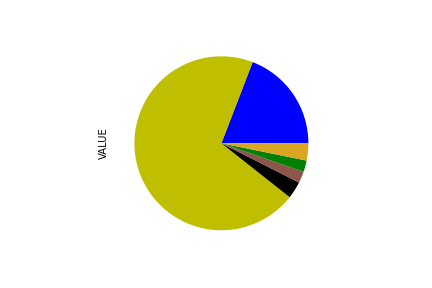
\includegraphics[width=\textwidth, trim={120pt 50pt 110pt 50pt}, clip]{../Ontario.png}%
\end{center}
\end{minipage}
\begin{center}
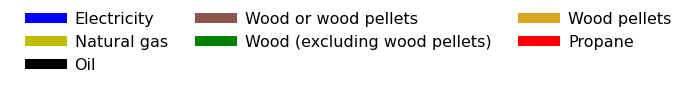
\includegraphics[width=0.8\linewidth]{leg_bar.png}
\end{center}

\begin{textblock*}{\textwidth}[0.5, 0.5](0.5\linewidth, 225pt)
\begin{itemize}
	\item SK, AB, and parts of BC have an extensive natural gas infrastructure.
	\item MB and ON have access to the natural gas TransCanada pipeline.
\end{itemize}
\end{textblock*}

\end{frame}






\begin{frame}
\frametitle{Cause of the Groupings: Electricity}
\vspace{-30pt}
\begin{center}
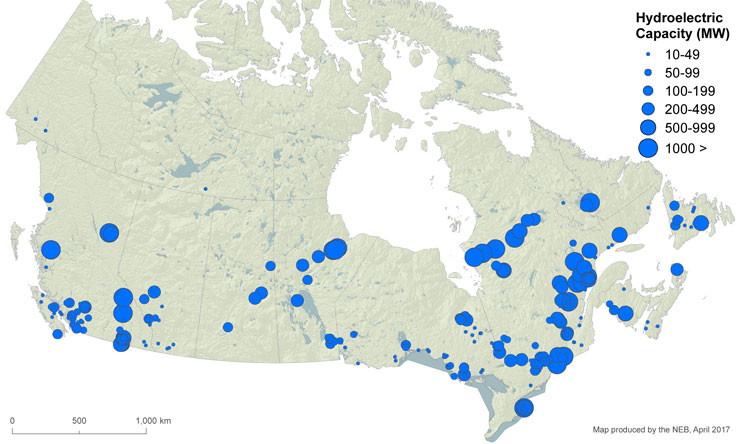
\includegraphics[width=0.8\textwidth]{hydroPower.jpg}
\end{center}

\begin{textblock*}{\textwidth}[0.5, 0.5](0.5\linewidth, 230pt)
\begin{itemize}
	\item QC: large hydroelectric capacity
	\item  NL and NB: close to QC, no access to natural gas  
\end{itemize}
\end{textblock*}
\end{frame}




\begin{frame}
\frametitle{Cause of the Groupings: Electricity}
\vspace{-25pt}
\begin{minipage}[b]{0.33\textwidth}
\begin{center}
Quebec
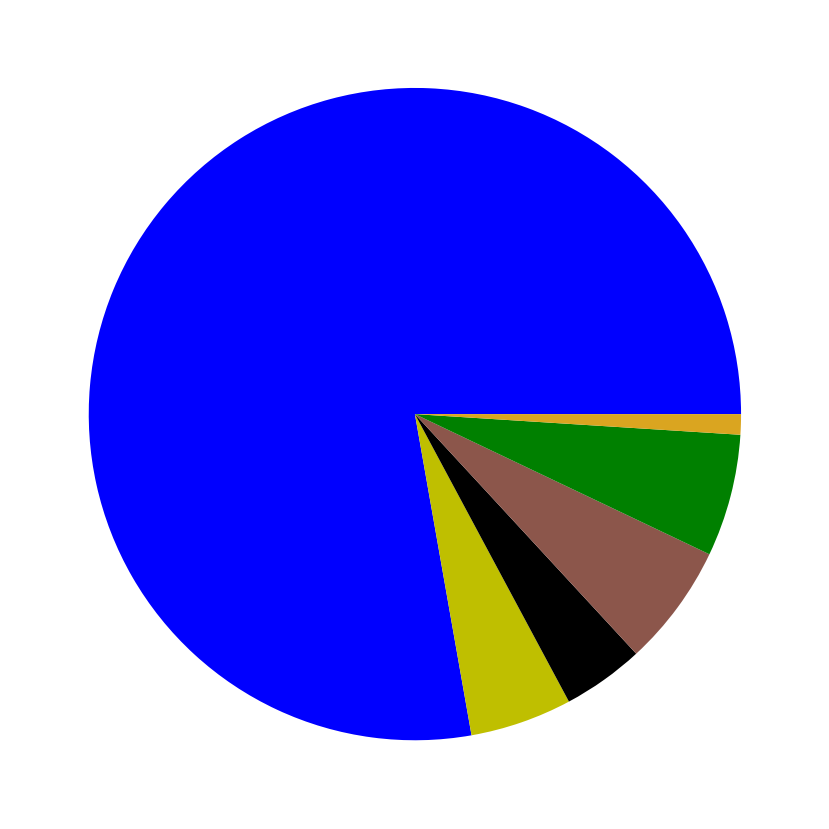
\includegraphics[width=\linewidth, trim={40pt 70pt 40pt 30pt}, clip]{Quebec2017.png}%
\end{center}
\end{minipage}%
%
\begin{minipage}[b]{0.33\textwidth}
\begin{center}
Newfoundland and Labrador
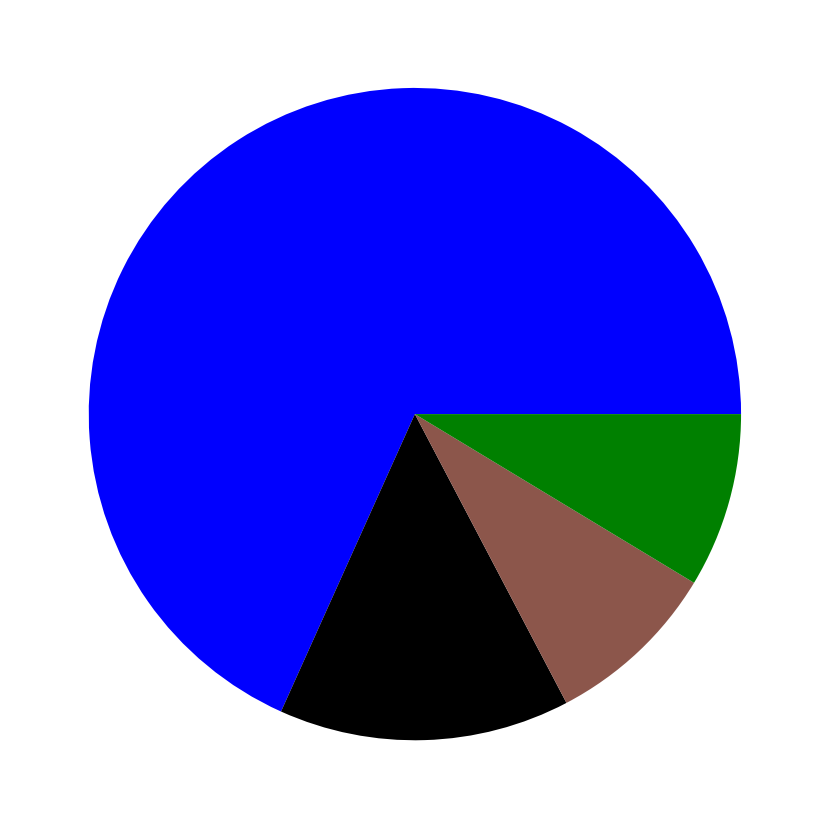
\includegraphics[width=\linewidth, trim={40pt 70pt 40pt 30pt}, clip]{NL2017.png}%
\end{center}
\end{minipage}%
%
\begin{minipage}[b]{0.33\textwidth}
\begin{center}
New Brunswick
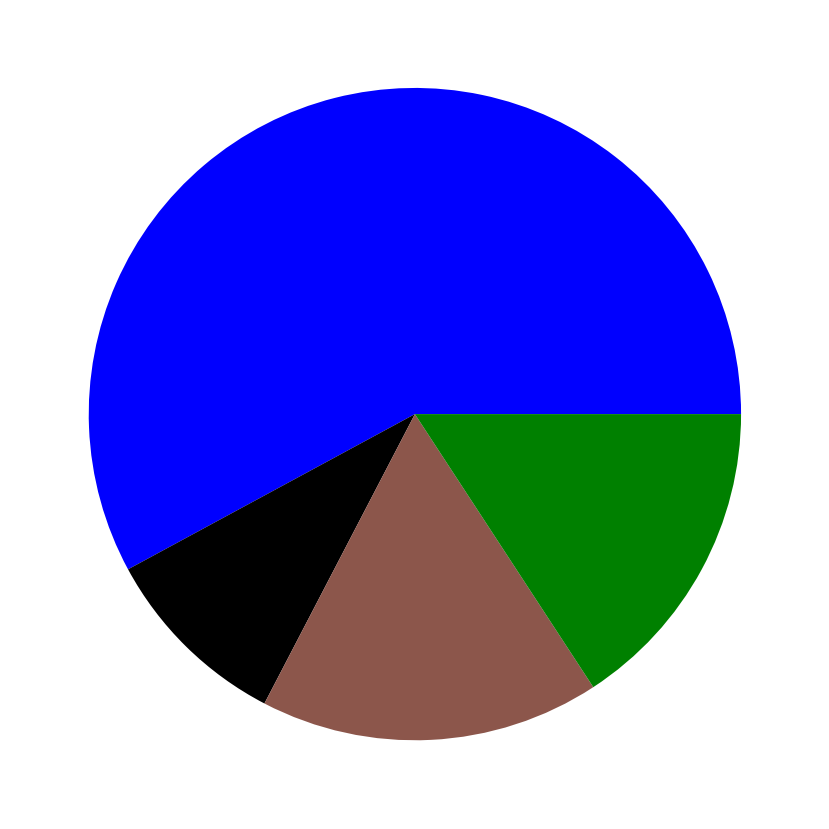
\includegraphics[width=\linewidth, trim={40pt 70pt 40pt 30pt}, clip]{NB2017.png}%
\end{center}
\end{minipage}



\begin{center}
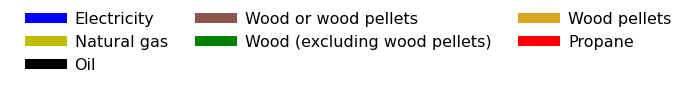
\includegraphics[width=0.8\linewidth]{leg_bar.png}
\end{center}


\begin{textblock*}{\textwidth}[0.5, 0.5](0.5\linewidth, 230pt)
\begin{itemize}
	\item QC: large hydroelectric capacity
	\item NL and NB: close to QC, no access to natural gas  
\end{itemize}
\end{textblock*}
\end{frame}











\begin{frame}
\frametitle{Cause of the Groupings: Atlantic Provinces}

\begin{center}
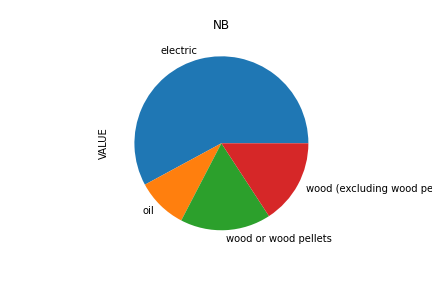
\includegraphics[width=0.25\linewidth, trim={120pt 50pt 110pt 10pt}, clip]{Ben_Images/NB.png}%
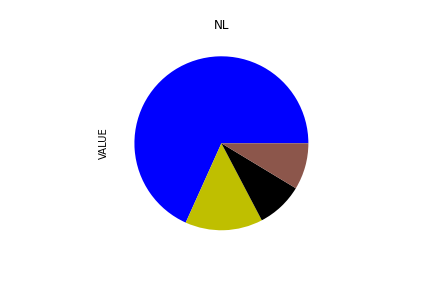
\includegraphics[width=0.25\linewidth, trim={120pt 50pt 110pt 10pt}, clip]{Ben_Images/NL.png}%
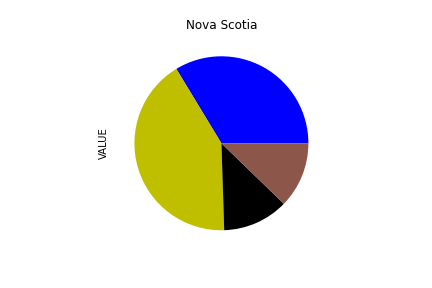
\includegraphics[width=0.25\linewidth, trim={120pt 50pt 110pt 10pt}, clip]{Ben_Images/NS.png}%
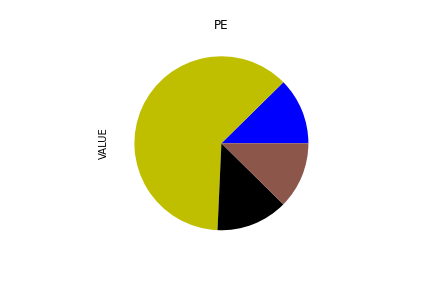
\includegraphics[width=0.25\linewidth, trim={120pt 50pt 110pt 10pt}, clip]{Ben_Images/PE.png}\\[10pt]
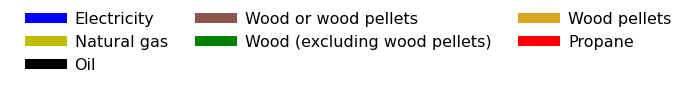
\includegraphics[width=0.8\linewidth]{leg_bar.png}
\end{center}

Same story in Atlantic region:
	\begin{itemize}
		\item Newfoundland, New Brunswick: access to hydro, use electric.
		\item Prince Edward Island, Nova Scotia: little hydro access, primarily oil.
	\end{itemize}

\end{frame}


















\begin{frame}
\frametitle{Summary}

\begin{itemize}

\item No change over time.

\item The dependence is predominantly geographic.

\end{itemize}


\begin{center}
\textbf{Thank you for your attention!}
\end{center}


\end{frame}













\end{document}
